\documentclass[answers]{exam}

\usepackage{amsmath}
\usepackage{amssymb}
\usepackage{geometry}
\usepackage{venndiagram}
\usepackage{graphics}
\usepackage{graphicx}
\usepackage{tikz}
\usepackage{listings}
\usepackage{subfig}
\usepackage{float}
\lstset{
    basicstyle=\ttfamily,
    columns=fullflexible,
    frame=single,
    breaklines=true,
    postbreak=\mbox{\textcolor{red}{$\hookrightarrow$}\space},
}

% Header and footer.
\pagestyle{headandfoot}
\runningheadrule
\runningfootrule
\runningheader{EE/CE 468/468 Mobile Robotics}{Homework 2}{Fall 2023}
\runningfooter{}{Page \thepage\ of \numpages}{}
\firstpageheader{}{}{}

\boxedpoints
\printanswers

\newcommand{\uvec}[1]{\boldsymbol{\hat{\textbf{#1}}}}
\newcommand\union\cup
\newcommand\inter\cap
\newcommand\ul\underline
\newcommand\ol\overline

\title{Assignment 2\\ EE/CE 468/468 Mobile Robotics\\ Habib University -- Fall 2023}
\author{Ali Asghar Yousuf \\ Muhammad Azeem Haider }  % replace with your ID, e.g. oy02945
\date{\today}

\begin{document}
\maketitle

\begin{questions}
    \question Problem 2
    \subsection*{Code}

    \begin{lstlisting}
    function [phiDotL, phiDotR] = wheelSpeed(v, omega, waypoints, pose)
        % Path constants
        stopThreshold = 0.1;
        slowThreshold = 0.3;
        
        % Robot constants
        trackWidth = 0.381;
        wheelRadius = 0.195/2;
        
        % Convert velocity and heading angular velocity to wheel speeds
        phiDotL = (v - trackWidth/2*omega)/wheelRadius;
        phiDotR = (v + trackWidth/2*omega)/wheelRadius;
    
    end
    \end{lstlisting}
    \question Problem 3
    \subsection*{Code}

    \begin{lstlisting}
    function [LinVel, AngVel] = pidPathFollower(Waypoints,Pose)
        persistent n;
        x = Pose(1);
        y = Pose(2);
        phi = Pose(3);
        R = [cos(phi) sin(phi); -sin(phi) cos(phi)];
    
        if (isempty(n))
            n = 2;
        end
        % Completed the path
        if n > length(Waypoints)
            LinVel = 0;
            AngVel = 0;
        else
    
        xg = Waypoints(n, 1);
        yg = Waypoints(n, 2);
        phig = Waypoints(n, 3);
    
        ep = R*([xg; yg]-[x; y]);
        xe = ep(1);
        ye = ep(2);
        epsilon = 0.02;
    
        if sqrt(ye^2 + xe^2) < epsilon
            n = n + 1;
        end

        % kp = 0;
        % kd = 0;
        
        % kp = 10;
        % kd = 0;

        % kp = 50;
        % kd = 0;

        % kp = 50;
        % kd = 10;

        % kp = 50;
        % kd = 0.5;
        
        kp = 60;
        kd = 0.08;
        LinVel = 0.2*xe + 0.1;
        K = kp*(ye) + kd*sin(phig - phi);
        AngVel = LinVel*K;
    
        end
    end
    \end{lstlisting}

    \subsection*{Discussion}
    I have added some graphs of when I was tuning the values of $k_p$ and $k_d$
    \begin{figure}[H]
        \centering
        \subfloat[$k_p = 0, k_d = 0$]{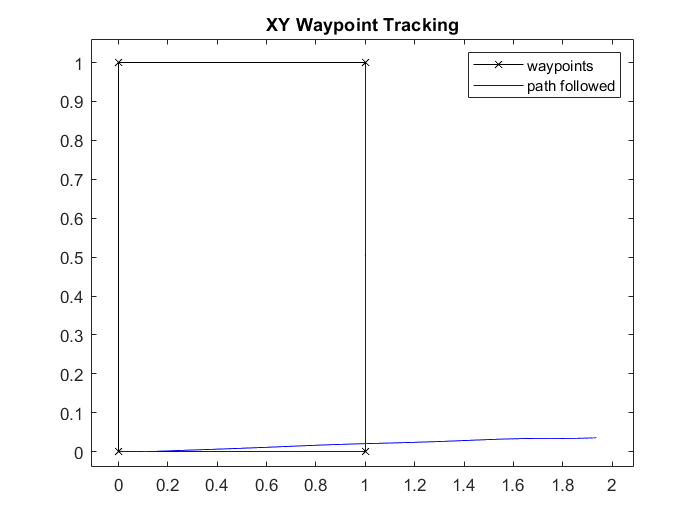
\includegraphics[width=0.3\columnwidth]{images/3-kd0kp0.png}}
        \qquad
        \subfloat[$k_p = 1, k_d = 0$]{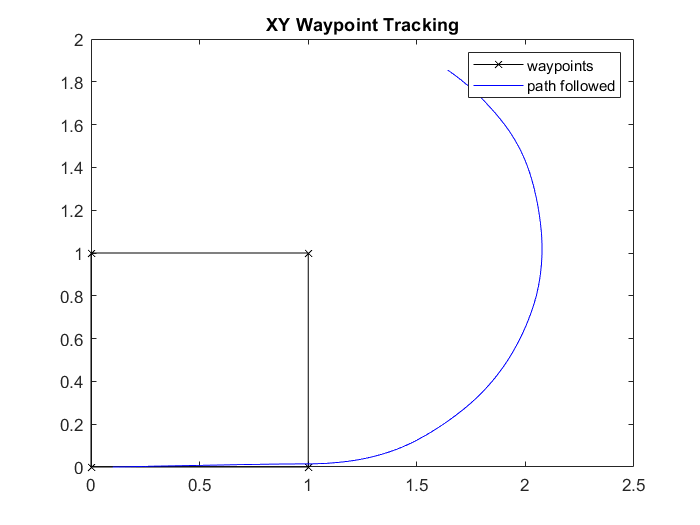
\includegraphics[width=0.3\columnwidth]{images/3-kd0kp1.png}}
        \qquad
        \subfloat[$k_p = 50, kd=0$]{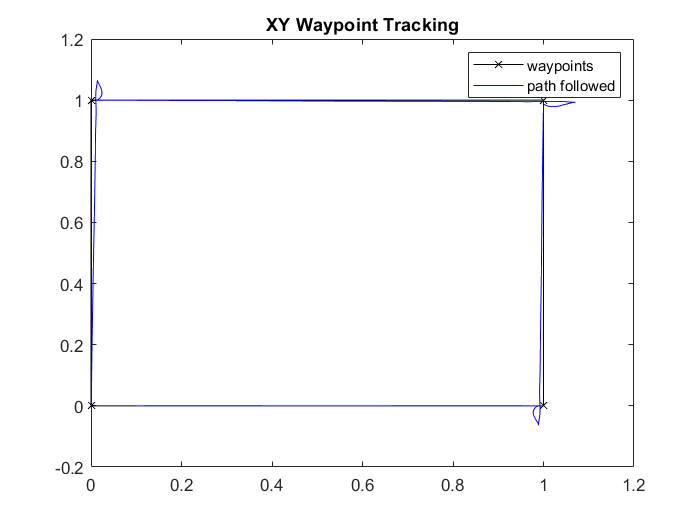
\includegraphics[width=0.3\columnwidth]{images/3-kd0kp50.png}}
        \label{fig:Comparison}\\

        \subfloat[$k_p = 50, k_d = 10$]{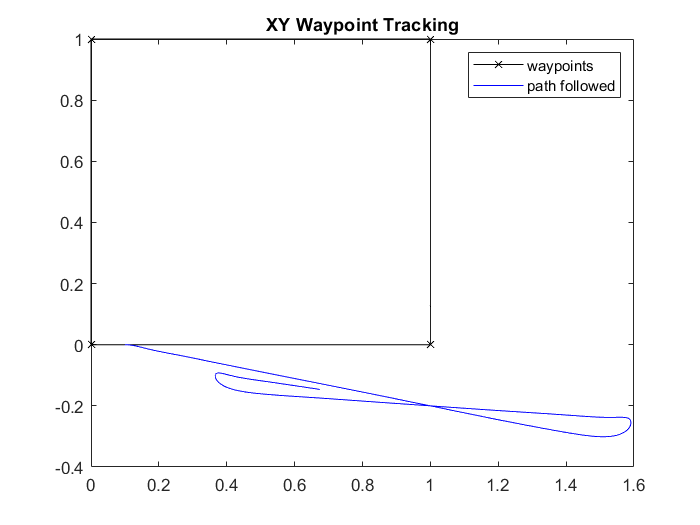
\includegraphics[width=0.3\columnwidth]{images/3-kd10kp50.png}}
        \qquad
        \subfloat[$k_p = 50, k_d = 2$]{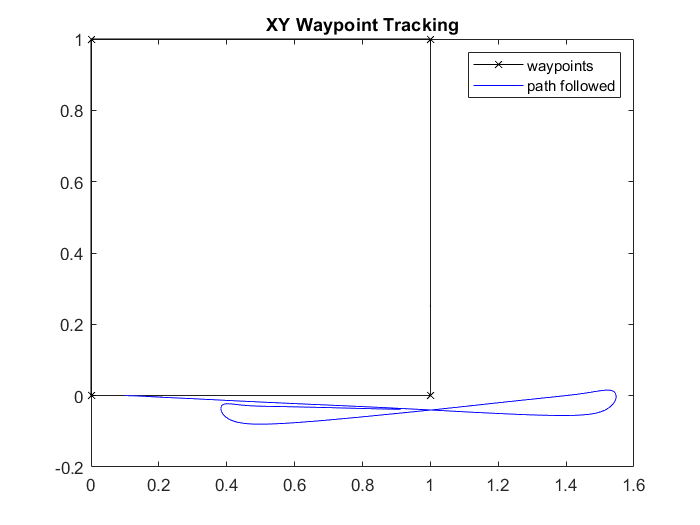
\includegraphics[width=0.3\columnwidth]{images/3-kd2kp50.png}}
        \qquad
        \subfloat[$k_p = 50, kd=0.5$]{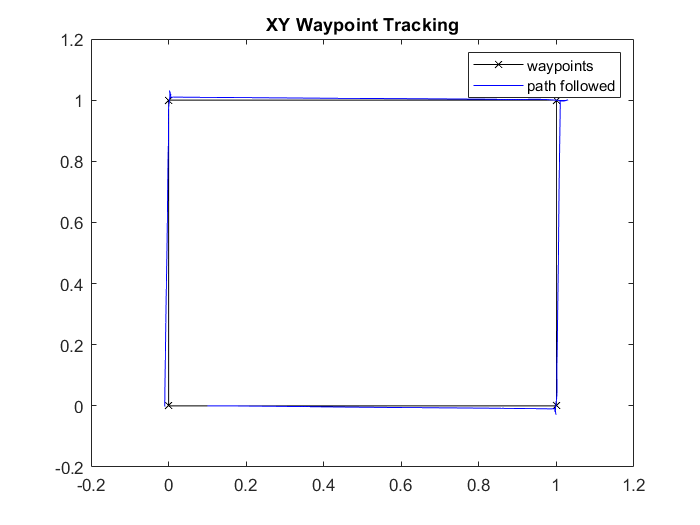
\includegraphics[width=0.3\columnwidth]{images/3-kd0.5kp50.png}}
        \label{fig:Comparison}\\
    \end{figure}

    I began with both $k_p$ and $k_d = 0$, then I started increasing $k_p$ as
    initially I was getting a very straight path, as I gradually increased $k_p$
    the path started converging to the waypoints.

    Similarly, after I had tuned $k_p$, I started with a high value of 10 as $k_p$
    converged at a higher value, but, this time around my path got even worse, so I
    realized that the value was too high, then I gradually started decreasing but
    it was not until I decreased $k_d$ below that I started getting some promising
    results.

    \subsection*{Waypoint Tracking}
    \begin{figure}[H]
        \centering
        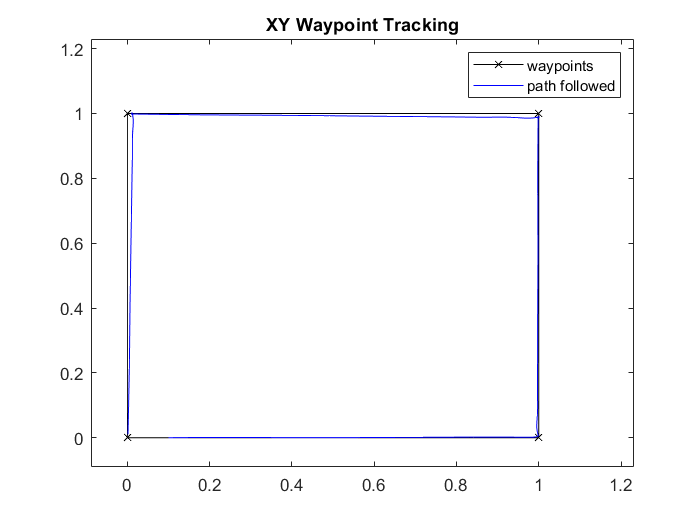
\includegraphics[width=0.8\textwidth]{images/3-square.png}
        \caption{PID Path Follower}
        \label{fig:my_label}
    \end{figure}

    \question Problem 4
    \subsection*{Discussion}
    The square in the previous problem was achieved with $\epsilon = 0.02$,
    however, that did not work too well with other shapes as it was overfitted for
    a square.
    \begin{figure}[H]
        \centering
        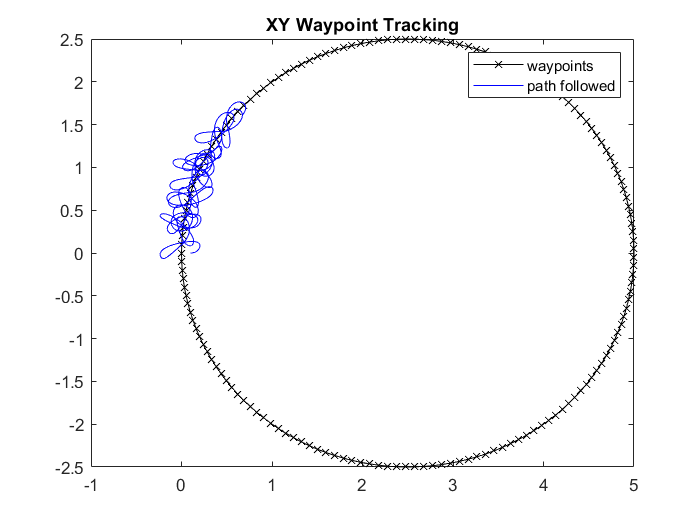
\includegraphics[width=0.4\textwidth]{images/4-circle-e.png}
        \caption{Circle with $\epsilon=0.02$}
        \label{fig:enter-label}
    \end{figure}

    Nonetheless, by increasing $\epsilon \text{ to } 0.11$ we were able to achieve
    some very good results. We observed that the robot had some trouble figuring
    out the path initially as it's orientation was different than the waypoints,
    but it was still able to perform very well once it was on track.
    \subsection*{Waypoint Tracking}
    \begin{figure}[H]
        \centering
        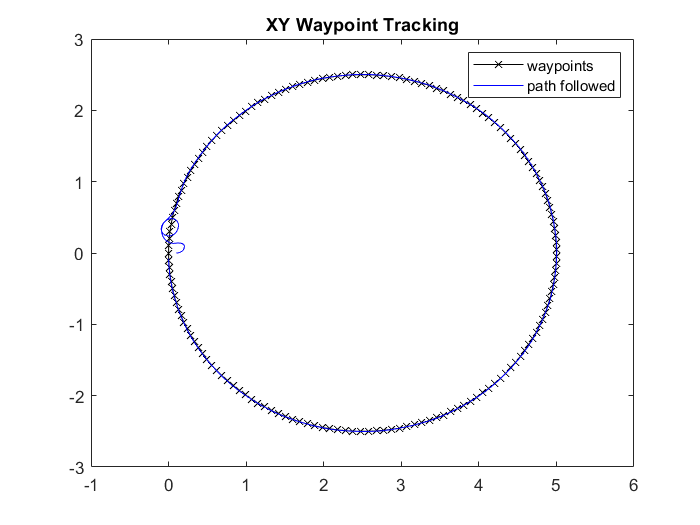
\includegraphics[width=0.8\textwidth]{images/4-circle.png}
        \caption{Circle}
        \label{fig:my_label}
    \end{figure}

    \begin{figure}[H]
        \centering
        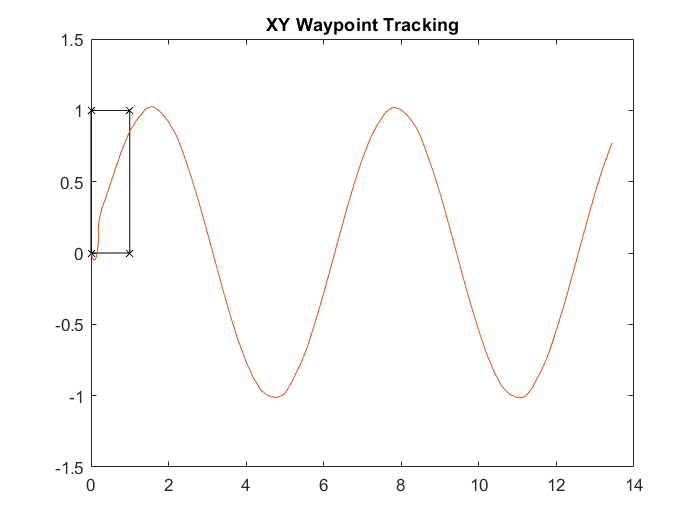
\includegraphics[width=0.8\textwidth]{images/4-wave.png}
        \caption{Wave}
        \label{fig:my_label}
    \end{figure}

    \question Problem 5
    \subsection*{Code}
    \begin{lstlisting}
    function [v, w] = PurePursuitPathFollower(Pose, WayPoints)
        % Define the lookahead distance
        lookahead_dist = 0.08;
    
        % Extract the heading angle from the pose
        phi = Pose(3);
        
        % Calculate trigonometric values for coordinate transformation
        cos_phi = cos(phi);
        sin_phi = sin(phi);
        
        % Create a rotation matrix for coordinate transformation
        Rot_Mat = [cos_phi, sin_phi; -sin_phi, cos_phi];
    
        % Initialize a persistent state variable to keep track of the current waypoint
        persistent n;
        if (isempty(n))
            n = 2; % Start with the second waypoint
        end
        
        % Check if all waypoints have been reached
        if n > length(WayPoints)
            v = 0; % Set linear velocity to zero
            w = 0; % Set angular velocity to zero
        else
            % Extract the current position
            x = Pose(1);
            y = Pose(2);
            
            % Calculate the slope of the line connecting the robot to the current waypoint
            m = (WayPoints(n,2) - y) / (WayPoints(n,1) - x);
            
            % Generate a set of angles to sample candidate goal points
            angles = 0:0.05*pi:2*pi;
            
            % Calculate x and y coordinates of candidate goal points
            x_cord = x + lookahead_dist * cos(angles);
            y_cord = y + lookahead_dist * sin(angles);
            
            % Calculate distances from the current waypoint to the candidate goal points
            if m == 0
                distances = abs(y_cord - y);
            elseif isinf(m)
                distances = abs(x_cord - x);
            else
                distances = abs(y_cord - m * x_cord - (WayPoints(n,2) - m*WayPoints(n,1)));
            end
            
            % Filter out candidate goal points that are too far from the path
            valid_indices = distances < 0.2;
            goal_pointx = x_cord(valid_indices);
            goal_pointy = y_cord(valid_indices);
    
            % Calculate the distances between candidate goal points and the current waypoint
            dists = sqrt((goal_pointx - WayPoints(n, 1)).^2 + (goal_pointy - WayPoints(n, 2)).^2);
            
            % Find the index of the minimum distance
            [min_d, min_idx] = min(dists);
            
            % Update the goal point based on the index of the minimum distance
            goal_point = [goal_pointx(min_idx); goal_pointy(min_idx)];
    
            % Extract the x and y coordinates of the current waypoint
            xg = WayPoints(n, 1);
            yg = WayPoints(n, 2);
            
            % Calculate the error in position relative to the current waypoint
            pose_diff = [xg; yg] - [x; y];
            
            % Transform the position error into the robot's local coordinate frame
            curr_error = Rot_Mat * pose_diff;
            x_curr_error = curr_error(1);
            y_curr_error = curr_error(2);
            
            % Calculate the Euclidean distance from the robot to the current waypoint
            d = sqrt(y_curr_error^2 + x_curr_error^2);
            
            % Define a small value for comparison
            epsilon = 0.02;
            
            % Determine robot velocity based on the position error
            if d > epsilon
                v = 0.3; % Set linear velocity
                goal_point_diff = goal_point - [Pose(1); Pose(2)];
                
                % Transform the goal point error into the robot's local coordinate frame
                trans_gpd = Rot_Mat * goal_point_diff;
                
                % Calculate steering angle based on the transformed error
                lambda = 2 * trans_gpd(2) / lookahead_dist^2;
                w = 0.5 * lambda; % Set angular velocity
            else
                % Proceed to the next waypoint
                n = n + 1;
                v = 0; % Set linear velocity to zero
                w = 0; % Set angular velocity to zero
            end
        end
    end
    \end{lstlisting}

    \subsection*{Discussion}
    The above \textit{Pure Pursuit path following} algorithm was tested on
    different values of look-ahead distance, linear velocity and the constant of
    angular velocity. Different metrics yielded different results. It is important
    to note that smaller values of look-ahead distance resulted in better results
    of the robot tracking the waypoints. However, only changing the look-ahead
    distance was not important, since the value of look-ahead distance was kept
    small, it was imperative that the linear velocity was not very high because
    that was resulting in bad tracking and almost skidding of the gazebo robot.
    This is why it is important that a combination of a small look-ahead distance
    value with a slow linear velocity. The angular velocity was also managed in a
    manner that did not result in sudden turns, and a higher constant resulted in
    the robot turning sharply which was resulting in inaccurate path following.

    \begin{figure}[H]
        \centering
        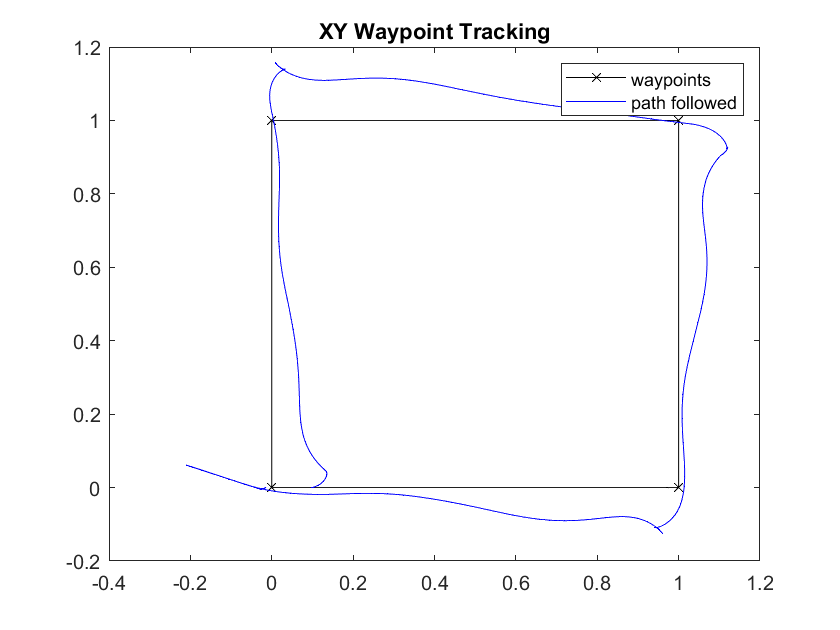
\includegraphics[width=0.7\textwidth]{images/5-discuss.png}
        \caption{This is robot tracking at a small look-ahead distance value 0.08 but a relatively bigger linear velocity of 1}
        \label{fig:my_label}
    \end{figure}

    \subsection*{Waypoint Tracking}

    \begin{figure}[H]
        \centering
        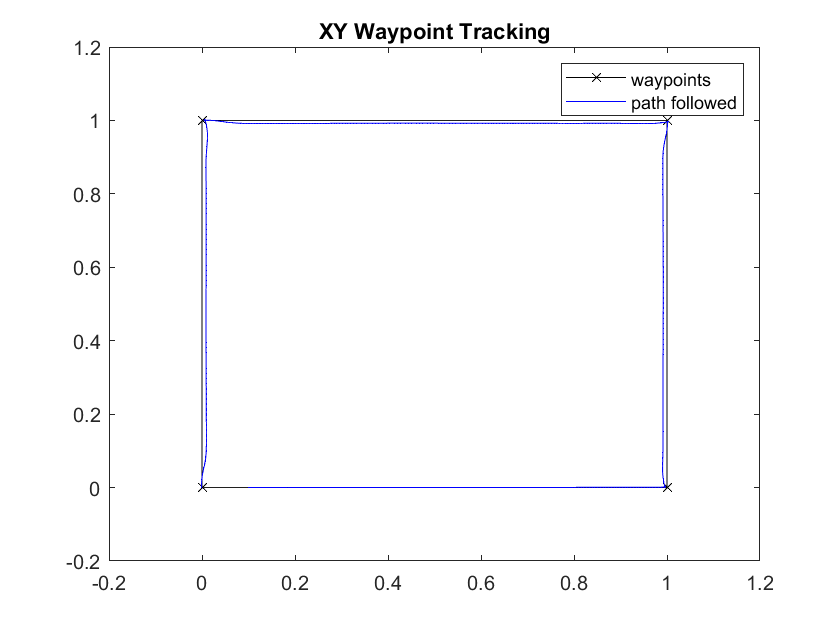
\includegraphics[width=0.7\textwidth]{images/5-square.png}
        \caption{Square}
        \label{fig:my_label}
    \end{figure}

    \begin{figure}[H]
        \centering
        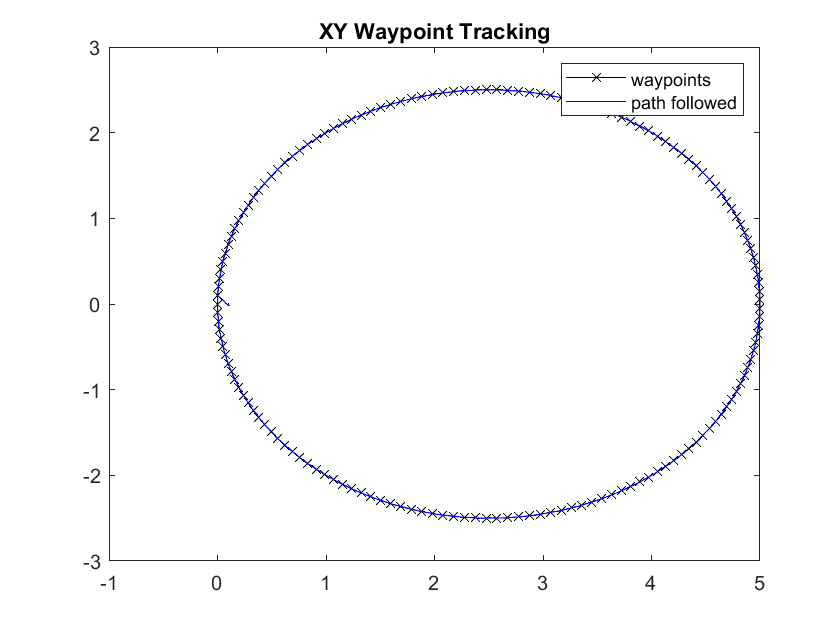
\includegraphics[width=0.8\textwidth]{images/5-circle.png}
        \caption{Circle}
        \label{fig:my_label}
    \end{figure}

    \begin{figure}[H]
        \centering
        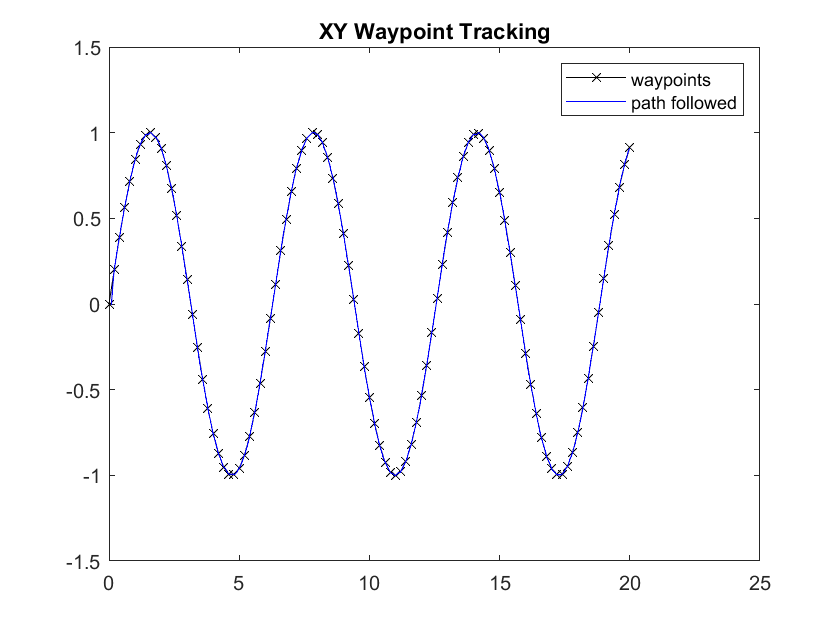
\includegraphics[width=0.8\textwidth]{images/5-wave.png}
        \caption{Wave}
        \label{fig:my_label}
    \end{figure}

    \question Problem 6
    \section*{Code}
    \begin{lstlisting}
    function odo_pose = Odometery(wheelSpeed)
        persistent x;
        persistent y;
        persistent phi;
        phiDotL = wheelSpeed(1);
        phiDotR = wheelSpeed(2);
        if isempty(x)
            x = 0;
            y = 0;
            phi = 0;
            odo_pose = [x; y; phi];
        else
            trackWidth = 0.381;
            wheelRadius = 0.195/2;
            LinVel = (phiDotL + phiDotR) * wheelRadius/2;
            AngVel = (phiDotR - phiDotL) * wheelRadius/trackWidth;
    
            x = x + (LinVel * 0.01/2 * (cos(phi) + cos(phi + 0.01 * AngVel)));
            y = y + (LinVel * 0.01/2 * (sin(phi) + sin(phi + 0.01 * AngVel)));
            phi = phi + 0.01 * AngVel;
            odo_pose = [x; y; phi;];
        end
    end
    \end{lstlisting}

    \subsection*{Waypoint Tracking}
    \begin{figure}[H]
        \centering
        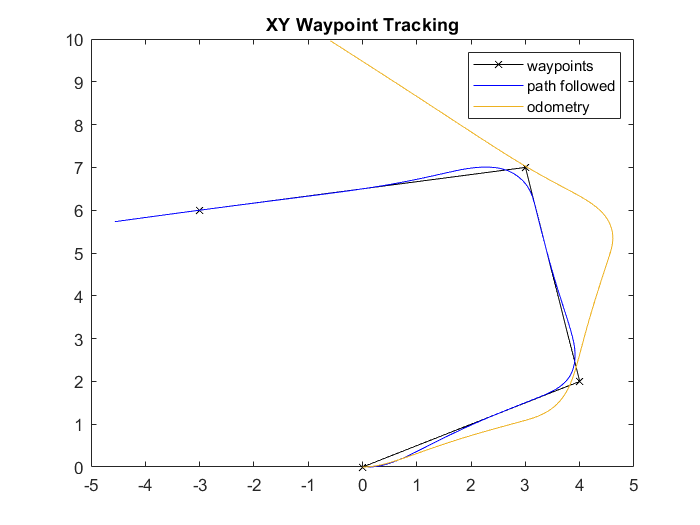
\includegraphics[width=0.8\textwidth]{images/6-default.png}
        \caption{Caption}
        \label{fig:enter-label}
    \end{figure}

    \subsection*{Discussion}
    We can see that using the default pure pursuit controller, our robot has
    followed the path correctly however the odometry is way off track. There are a
    couple of notable observations that can be made from the graph.
    \begin{enumerate}
        \item The initial straight path of odometry to the 1st waypoint is not that off
              track, however when the robot turns i.e the angular velocity increases, the
              sensors are unable to accurately measure that which leads to the cross-track
              error. Once again as the robot turns, the odometry shown has an angle lesser
              than the actual robot path
        \item On the second hand, we see little error along the direction of the robot i.e
              the straight paths taken by the robot are similar in length to those of the
              intended path.
    \end{enumerate}

    \question Problem 7
    \subsection*{Discussion}
    We observed that the shape tracked by the robot was almost the same for the
    circle and the wave as the intended path, however, both were translated a
    little. We also observed that the error in the measurement was increasing which
    was more visible in the wave.

    As for the square, we saw similar behavior from the odometry from the previous
    part, it underestimated the angular velocity of the robot which resulted in the
    robot turning more than it should. \subsubsection*{Waypoint Tracking}
    \begin{figure}[H]
        \centering
        \subfloat[PID Circle]{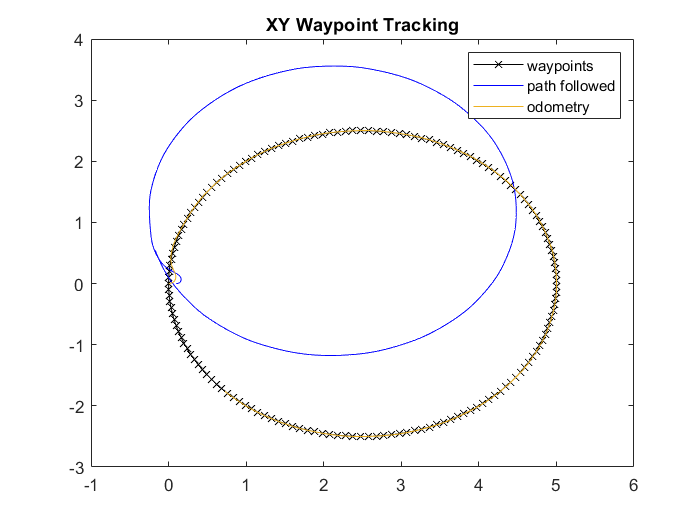
\includegraphics[width=0.45\columnwidth]{images/7-pid-circle.png}}
        \qquad
        \subfloat[PID Square]{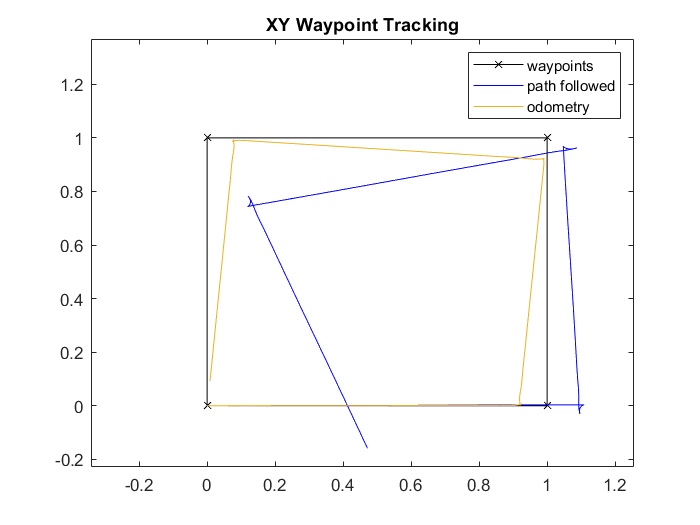
\includegraphics[width=0.45\columnwidth]{images/7-pid-square.png}}\\
        \subfloat[PID Wave]
        {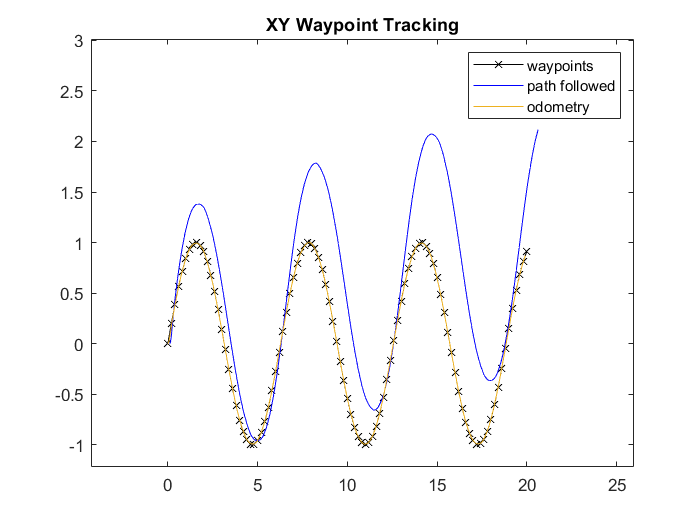
\includegraphics[width=0.45\columnwidth]{images/7-pid-wave.png}}
    \end{figure}
    \question Problem 8
    \begin{parts}
        \part Part a
        \begin{solution}
            \subsection*{Ali Asghar Yousuf}
            20 hours
            \subsection*{Muhammad Azeem Haider}
            22 hours

        \end{solution}
        \part Part b
        \begin{solution}
            \subsection*{Ali Asghar Yousuf}
            \begin{enumerate}
                \item Q1
                \item Q3
                \item Q4
                \item Q6
            \end{enumerate}

            \subsection*{Muhammad Azeem Haider}
            \begin{enumerate}
                \item Q1
                \item Q2
                \item Q5
                \item Q7
            \end{enumerate}
        \end{solution}
        \part Part c
        \begin{solution}
            \subsection*{Ali Asghar Yousuf}
            I applied my understanding of pid controllers to attempt problems 3 and 4. The
            velocities of robot $(v, \omega)$ depend on the error in position and the
            heading angle. As for problem 6, I applied my understanding of the kinematics
            of a differential drive robot to calculate the linear and angular velocities of
            the robot and use that to calculate the pose of the robot.

            \begin{itemize}
                \item I faced a number of challenges while attempting this homework, the first one
                      was obviously figuring out MATLAB as it was my first time using it. Setting up
                      gazebo was pretty simple as compared to my preconceived notions.
                \item I was pretty confused about the PID controller at first, but after reading the
                      slides and asking some friends, I was able to understand the concept and
                      implement it.
            \end{itemize}
            \subsection*{Muhammad Azeem Haider}
            The bulk of my time in this homework was spent on first figuring out how to
            setup Matlab with gazebo simulator, once that was done, the second biggest
            challenge was writing Pure Pursuit Path Following algorithm. The research paper
            from Carnegie Mellon University explains the algorithm in a simple manner but
            it proved to be a time consuming task because I was unable to figure out what
            was the best way to calculate the distance from the current position to the
            goal position. Question 7 was comparatively simpler but the result achieved was
            not as good because of the sensors used in Matlab I believe. I would still want
            to brush up prior concepts that were used in the Pure Pursuit Path Following
            algorithm.
        \end{solution}
    \end{parts}

\end{questions}

\end{document}